% ============================================================================
%  Erdos Problem 915 -- 60-minute seminar deck
%  Built directly from the figures, tables and theorems pasted into this file.
%  Self-contained: no dependency on ../thesis-beamer.tex or ../../shared/,
%  since this file lives one directory deeper than those.
%  Build:  cd slides/seminarie && latexmk -pdf main.tex
% ============================================================================
\documentclass[aspectratio=1610,11pt]{beamer}

\usepackage[T1]{fontenc}
\usepackage[utf8]{inputenc}
\usepackage{helvet}
\renewcommand{\familydefault}{\sfdefault}
\usepackage{amsmath,amssymb}
\usepackage{booktabs}
\usepackage{array}
\usepackage{multirow}
\usepackage{tabularx}
\usepackage{graphicx}
\usepackage{adjustbox}
\usepackage{tikz}
\usetikzlibrary{calc,arrows.meta,positioning,backgrounds,fit,shadows,decorations.markings}

\graphicspath{{../../figures/}{../../}}

% ============================================================================
%  COLOURS  (KU Leuven palette + the thesis's semantic graph colours)
% ============================================================================
\definecolor{KULblauw1}{RGB}{29,141,176}
\definecolor{KULblauw3a}{RGB}{82,189,236}
\definecolor{KULblauw3b}{RGB}{30,110,135}
\definecolor{vertexred}{RGB}{200,80,80}
\definecolor{vertexpurple}{RGB}{140,80,160}
\definecolor{vertexgreen}{RGB}{60,160,80}
\definecolor{vertexorange}{RGB}{220,140,40}

\definecolor{metroA}{RGB}{200,80,80}
\definecolor{metroB}{RGB}{29,141,176}
\definecolor{metroC}{RGB}{60,160,80}
\definecolor{metroD}{RGB}{220,140,40}
\definecolor{metroE}{RGB}{140,80,160}
\definecolor{metroF}{RGB}{120,120,120}

\definecolor{roleModel}{RGB}{82,189,236}
\definecolor{roleMeasure}{RGB}{29,141,176}
\definecolor{roleProve}{RGB}{60,160,80}
\definecolor{roleDiscover}{RGB}{220,140,40}

\colorlet{regimeProved}{KULblauw1}
\colorlet{regimeConjectured}{vertexred}
\colorlet{regimeOpen}{vertexorange}
\colorlet{regimePartial}{vertexpurple}

\definecolor{vtProved}{HTML}{1D8DB0}
\definecolor{vtConjectured}{HTML}{E05050}
\definecolor{vtOpen}{HTML}{E6B800}
\definecolor{vtExact}{HTML}{3CA050}
\definecolor{vtSearch}{HTML}{9B5DE5}

% ============================================================================
%  THE CANONICAL THESIS GRAPH VOCABULARY  (copied from preamble.tex)
% ============================================================================
\tikzset{
  gvertex/.style={circle, draw=KULblauw1, fill=KULblauw1!15, line width=1pt,
                  minimum size=6mm, inner sep=0pt, font=\small,
                  drop shadow={shadow xshift=0.4pt, shadow yshift=-0.5pt,
                               fill=black, opacity=0.18}},
  gline/.style ={line width=1.3pt, KULblauw1!75, line cap=round},
  gfaint/.style={line width=0.9pt, KULblauw1!40, line cap=round},
  gvhub/.style ={gvertex, draw=vertexorange, fill=vertexorange!18},
  gvsink/.style={gvertex, draw=vertexred,    fill=vertexred!15},
  gvcut/.style ={gvertex, draw=vertexpurple, fill=vertexpurple!20},
  gvnew/.style ={gvertex, draw=vertexorange, fill=vertexorange!22},
  gmulti/.style={gline},
  gdir/.style     ={-{Stealth[length=2.2mm]}, line width=1.1pt, KULblauw1!75, line cap=round},
  gdirfaint/.style={-{Stealth[length=1.8mm]}, line width=0.8pt, KULblauw1!40, line cap=round},
  gcut/.style     ={-{Stealth[length=2.2mm]}, line width=1.2pt, densely dashed, vertexred},
  gcutedge/.style ={line width=1.2pt, densely dashed, vertexred},
  grA/.style={line width=2.6pt, vertexorange,        line cap=round},
  grB/.style={line width=2.6pt, vertexgreen!70!black, line cap=round},
  grC/.style={line width=2.6pt, vertexpurple,         line cap=round},
  grAd/.style={grA, -{Stealth[length=2.8mm]}},
  grBd/.style={grB, -{Stealth[length=2.8mm]}},
  grCd/.style={grC, -{Stealth[length=2.8mm]}},
  gcurve/.style ={bend left=14},
  gcurveR/.style={bend right=14},
  vertex/.style={gvertex},
  smallvertex/.style={gvertex, minimum size=16pt, font=\scriptsize},
  edge/.style={gline},
  arc/.style={gdir},
  metro/.style={line width=3.4pt, line cap=round, line join=round, rounded corners=4pt},
  metrostop/.style={circle, draw=black!72, fill=white, line width=1pt,
                     minimum size=6mm, inner sep=0pt, font=\scriptsize\bfseries},
  hnode/.style={rectangle, draw=KULblauw3b, fill=white, minimum size=13pt,
                inner sep=1pt, line width=1pt, font=\scriptsize\bfseries},
  vtroot/.style={rectangle, rounded corners=3pt, draw=KULblauw3b, very thick,
                 minimum width=26mm, minimum height=9mm, font=\sffamily\small\bfseries},
  vtmodel/.style={rectangle, rounded corners=3pt, draw=KULblauw3b, thick,
                  minimum width=20mm, minimum height=8mm, font=\sffamily\small},
  vtdir/.style={rectangle, rounded corners=2.5pt, draw=KULblauw3b!70,
                minimum width=19mm, minimum height=7mm, font=\scriptsize},
  vtleaf/.style={rectangle, rounded corners=2pt, draw=KULblauw3b!70,
                 minimum width=12mm, minimum height=6.5mm, font=\scriptsize},
  vtedge/.style={KULblauw3b!55, line width=0.9pt},
}

% ============================================================================
%  NOTATION SHORTHANDS  (copied from preamble.tex)
% ============================================================================
\newcommand*{\floor}[1]{\left\lfloor #1 \right\rfloor}
\newcommand*{\floorfrac}[2]{\floor{\frac{#1}{#2}}}
\newcommand{\lec}{\lambda}
\newcommand{\kap}{\kappa}
\newcommand{\HH}{\mathcal{H}}
\newtheorem{proposition}{Proposition}
% carried over from ../../preamble.tex: marks a result whose proof here was
% written by an AI model and not checked line by line by the author.
\newcommand{\aimedal}{\,[AI]}

% ============================================================================
%  THEME
% ============================================================================
\setbeamertemplate{navigation symbols}{}
\usefonttheme{professionalfonts}
\setbeamercolor{structure}{fg=KULblauw1}
\setbeamercolor{frametitle}{fg=KULblauw3b}
\setbeamercolor{title}{fg=KULblauw3b}
\setbeamercolor{normal text}{fg=black!88}
\setbeamercolor{itemize item}{fg=KULblauw1}
\setbeamerfont{frametitle}{series=\bfseries,size=\large}
\setbeamerfont{title}{series=\bfseries}
\setbeamertemplate{itemize item}{\small\raise0.5pt\hbox{\textbullet}}

\setbeamertemplate{frametitle}{%
  \vskip4pt%
  \begin{beamercolorbox}[wd=\paperwidth,leftskip=0.9cm,rightskip=0.9cm]{frametitle}%
    \usebeamerfont{frametitle}\insertframetitle%
  \end{beamercolorbox}%
  \vskip2pt%
  \hspace*{0.9cm}{\color{KULblauw3a}\rule{0.82\paperwidth}{1.1pt}}%
  \vskip1pt%
}

\setbeamertemplate{footline}{%
  \hbox{%
    \begin{beamercolorbox}[wd=0.72\paperwidth,ht=2.4ex,dp=1.2ex,leftskip=0.9cm]{}%
      {\scriptsize\color{black!45}Erd\H{o}s{} Problem 915}%
    \end{beamercolorbox}%
    \begin{beamercolorbox}[wd=0.28\paperwidth,ht=2.4ex,dp=1.2ex,rightskip=0.9cm]{}%
      \hfill{\scriptsize\color{black!45}\insertframenumber\,/\,\inserttotalframenumber}%
    \end{beamercolorbox}%
  }%
}
\setbeamersize{text margin left=0.9cm,text margin right=0.9cm}

% ============================================================================
%  FRAME BUILDERS
% ============================================================================
\newcommand{\figframe}[3]{%
  \begin{frame}{#1}
    \vfill
    \begin{center}
    \includegraphics[width=\textwidth,height=0.66\textheight,keepaspectratio]{#2}
    \end{center}
    \vspace{3pt}
    \noindent{\footnotesize\color{black!60} #3}\par
    \vfill
  \end{frame}%
}
\newcommand{\figframetall}[3]{%
  \begin{frame}{#1}
    \vspace{-2pt}
    \begin{center}
    \includegraphics[width=\textwidth,height=0.66\textheight,keepaspectratio]{#2}
    \end{center}
    \vspace{1pt}
    \noindent{\tiny\color{black!60} #3}\par
  \end{frame}%
}
\newcommand{\tikzframescaled}[4]{%
  \begin{frame}{#1}
    \vfill
    \begin{center}
    \adjustbox{max totalheight=0.64\textheight}{\resizebox{#4\textwidth}{!}{#2}}
    \end{center}
    \vspace{8pt}
    \noindent{\footnotesize\color{black!60} #3}\par
    \vfill
  \end{frame}%
}
\newcommand{\tikzframe}[3]{\tikzframescaled{#1}{#2}{#3}{1.0}}

\title{Maximizing Edge Density Subject to Connectivity Constraints}
\author{Louis Vandenbruwaene}
\date{Academic Year 2026--2027}

\begin{document}

% ============================================================================
\begin{frame}[plain]
\vspace{1.9cm}
\hspace*{0.5cm}\begin{minipage}{0.9\textwidth}
  {\color{black!40}\large EXTREMAL GRAPH THEORY}\\[10pt]
  {\color{KULblauw3b}\fontsize{32}{36}\selectfont\bfseries Erd\H{o}s{} Problem 915}\\[8pt]
  {\color{KULblauw1}\Large Maximizing Edge Density Subject to Connectivity Constraints}\\[4pt]
  {\color{black!45}\small One-hour version}

  \vspace{1.4cm}
  {\large\bfseries Louis Vandenbruwaene}\\[3pt]
  {\small\color{black!70}Supervisor: Prof.\ Stijn Cambie \qquad Promotor: Prof.\ Jan Goedgebeur}\\[2pt]
  {\small\color{black!70}KU Leuven, Master of Mathematics}
\end{minipage}
\begin{tikzpicture}[remember picture,overlay]
  \node[anchor=south east] at ($(current page.south east)+(-0.8,0.5)$)
    {
\includegraphics[height=1.0cm]{LogoKULeuven.png}};
\end{tikzpicture}
\end{frame}

% ============================================================================
%  fig:k5-example
% ============================================================================
\tikzframe{The graph $K_5 - \{04,13\}$}{%
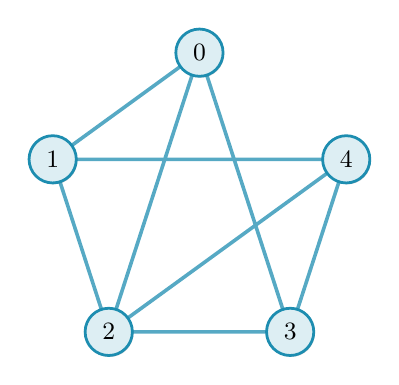
\begin{tikzpicture}[scale=1.4,
    mv/.style={gvertex},
    me/.style={gline}]
  \foreach \i in {0,...,4} {
    \pgfmathsetmacro{\ang}{90 + 72*\i}
    \coordinate (v\i) at (\ang:1.4);
  }
  \draw[me] (v0)--(v1) (v0)--(v2) (v0)--(v3)
            (v1)--(v2) (v1)--(v4)
            (v2)--(v3) (v2)--(v4)
            (v3)--(v4);
  \foreach \i in {0,...,4} {
    \pgfmathsetmacro{\ang}{90 + 72*\i}
    \node[mv] at (\ang:1.4) {$\i$};
  }
\end{tikzpicture}}{%
The simple graph $K_5-\{04,13\}$ has five vertices and eight edges, where $K_n$ is the complete graph on $n$ vertices.}

% ============================================================================
%  fig:menger
% ============================================================================
\tikzframe{Menger's theorem}{%
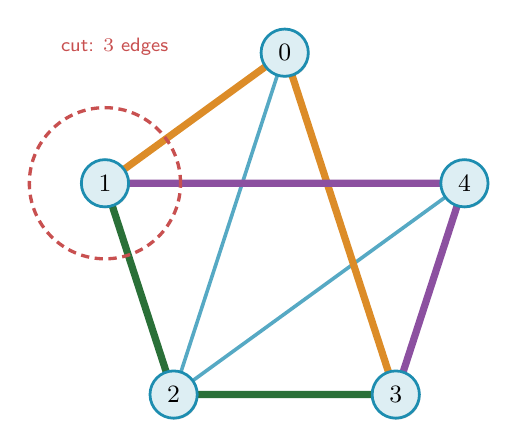
\begin{tikzpicture}[scale=1.6,
    mv/.style={gvertex},
    me/.style={gline},
    rA/.style={grA},
    rB/.style={grB},
    rC/.style={grC},
    cut/.style={gcutedge}]
  \foreach \i in {0,...,4} {
    \pgfmathsetmacro{\ang}{90 + 72*\i}
    \coordinate (v\i) at (\ang:1.5);
  }
  \draw[me] (v0)--(v1) (v0)--(v2) (v0)--(v3)
            (v1)--(v2) (v1)--(v4)
            (v2)--(v3) (v2)--(v4)
            (v3)--(v4);
  \draw[rA] (v1)--(v0)--(v3);
  \draw[rB] (v1)--(v2)--(v3);
  \draw[rC] (v1)--(v4)--(v3);
  \draw[cut] (v1) circle (0.6);
  \node[vertexred, font=\scriptsize] at (-1.35,1.55) {cut: $3$ edges};
  \foreach \i in {0,...,4} {
    \pgfmathsetmacro{\ang}{90 + 72*\i}
    \node[mv] at (\ang:1.5) {$\i$};
  }
\end{tikzpicture}}{%
Menger's theorem on $K_5-\{04,13\}$: three edge-disjoint $1$--$3$ routes (coloured) meet the minimal three-edge cut around vertex $1$, so $\lec(1,3)=3$.}

% ============================================================================
%  fig:directed-lambda
% ============================================================================
\tikzframe{Directed connectivity}{%
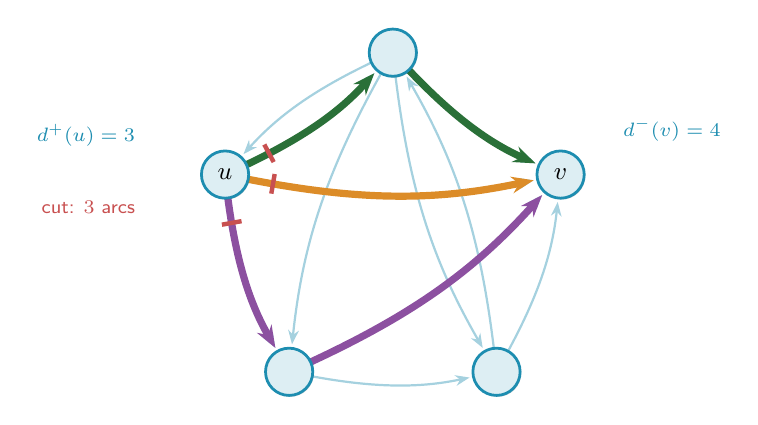
\begin{tikzpicture}[>=Stealth, scale=1.4,
    mv/.style={gvertex},
    me/.style={gdirfaint, shorten >=3.5mm},
    rA/.style={grAd, shorten >=3.5mm},
    rB/.style={grBd, shorten >=3.5mm},
    rC/.style={grCd, shorten >=3.5mm},
    cut/.style={gcutedge}]
\foreach \i in {0,...,4}{
    \pgfmathsetmacro{\ang}{90+72*\i}
    \coordinate (v\i) at (\ang:1.6);
}
\draw[me] (v1) to[bend right=12] (v0);
\draw[me] (v1) to[bend right=12] (v2);
\draw[me] (v1) to[bend right=12] (v4);
\draw[me] (v0) to[bend right=12] (v4);
\draw[me] (v2) to[bend right=12] (v4);
\draw[me] (v3) to[bend right=12] (v4);
\draw[me] (v0) to[bend right=12] (v2);
\draw[me] (v0) to[bend right=12] (v3);
\draw[me] (v3) to[bend right=12] (v0);
\draw[me] (v2) to[bend right=12] (v3);
\draw[rA] (v1) to[bend right=12] (v4);
\draw[me] (v0) to[bend right=12] (v1);
\draw[rB] (v1) to[bend right=12] (v0);
\draw[rB] (v0) to[bend right=12] (v4);
\draw[rC] (v1) to[bend right=12] (v2);
\draw[rC] (v2) to[bend right=12] (v4);
\tikzset{cuttick/.style={postaction={decorate, decoration={markings,
   mark=at position 0.62cm with {\draw[vertexred, line width=1.6pt]
        (0,-3.6pt) -- (0,3.6pt);}}}}}
\path[cuttick] (v1) to[bend right=12] (v4);
\path[cuttick] (v1) to[bend right=12] (v0);
\path[cuttick] (v1) to[bend right=12] (v2);
\node[vertexred, font=\scriptsize, anchor=east]
  at (-2.25, 0.2) {cut: $3$ arcs};
\node[font=\scriptsize, KULblauw1, anchor=east]
  at (-2.25, 0.85) {$d^{+}(u)=3$};
\node[font=\scriptsize, KULblauw1, anchor=west]
  at (2.0, 0.9) {$d^{-}(v)=4$};
\node[mv] at (v0) {};
\node[mv] at (v1) {$u$};
\node[mv] at (v2) {};
\node[mv] at (v3) {};
\node[mv] at (v4) {$v$};
\end{tikzpicture}}{%
Three arc-disjoint $u\to v$ routes (coloured) and the matching three-arc directed cut (red) in a simple digraph. Thus $\lambda(u,v)=3$, meeting the degree bound $\min(d^+(u),d^-(v))=3$.}

% ============================================================================
%  fig:eight-models
% ============================================================================
\begin{frame}{The eight models}
\vspace{-4pt}
\begin{center}
\adjustbox{max totalheight=0.60\textheight}{\resizebox{\textwidth}{!}{%
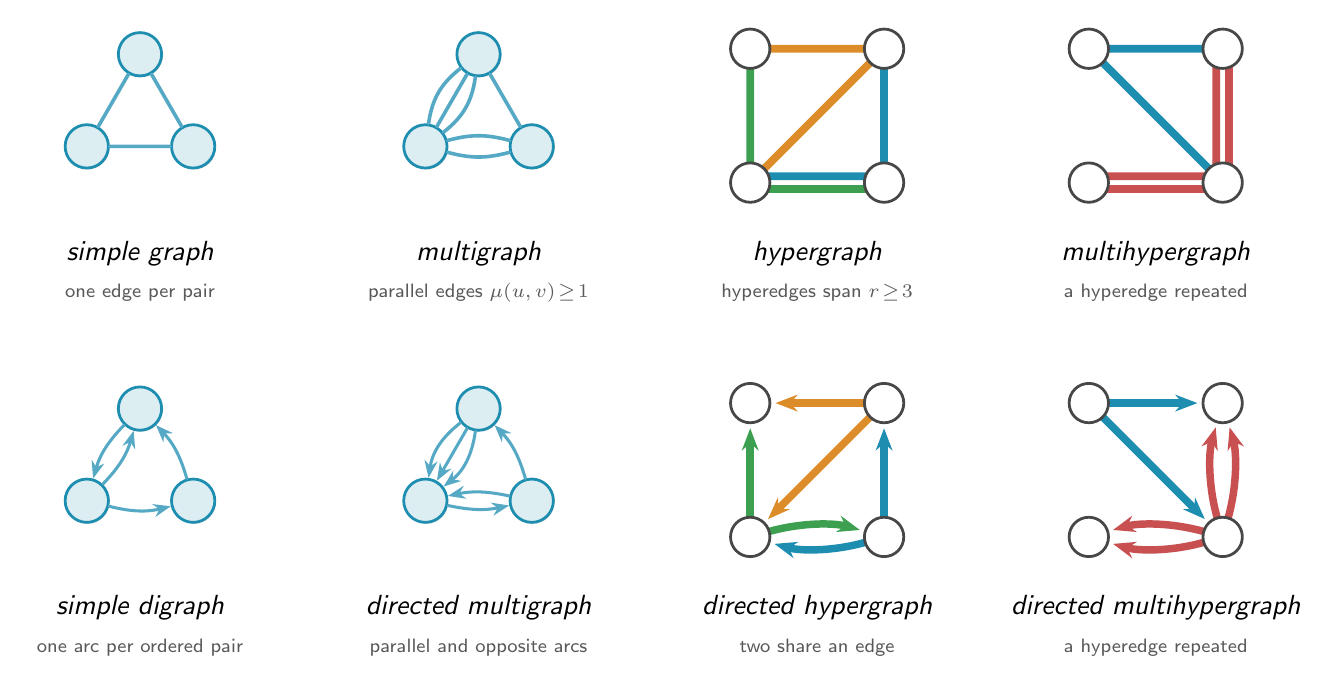
\begin{tikzpicture}[>=Stealth,
    mv/.style={gvertex, minimum size=5.5mm},
    me/.style={gline},
    ml/.style={metro, line width=2.8pt},
    stn/.style={metrostop, minimum size=5mm},
    darc/.style={gdir},
    hstar/.style={metro, line width=2.7pt, -{Stealth[length=2.8mm]}, shorten >=3.2mm, shorten <=2.4mm}]
  \begin{scope}[shift={(0,0)}]
    \node[mv] (s1) at (90:0.78) {};
    \node[mv] (s2) at (210:0.78) {};
    \node[mv] (s3) at (330:0.78) {};
    \draw[me] (s1)--(s2)  (s2)--(s3)  (s3)--(s1);
    \node[font=\itshape] at (0,-1.75) {simple graph};
    \node[font=\scriptsize, text=black!65] at (0,-2.25) {one edge per pair};
  \end{scope}
  \begin{scope}[shift={(4.30,0)}]
    \node[mv] (g1) at (90:0.78) {};
    \node[mv] (g2) at (210:0.78) {};
    \node[mv] (g3) at (330:0.78) {};
    \draw[me] (g1) to[bend left=22] (g2);
    \draw[me] (g1) -- (g2);
    \draw[me] (g1) to[bend right=22] (g2);
    \draw[me] (g2) to[bend left=15] (g3);
    \draw[me] (g2) to[bend right=15] (g3);
    \draw[me] (g3) -- (g1);
    \node[font=\itshape] at (0,-1.75) {multigraph};
    \node[font=\scriptsize, text=black!65] at (0,-2.25) {parallel edges $\mu(u,v)\!\ge\!1$};
  \end{scope}
  \begin{scope}[shift={(8.60,0)}]
    \coordinate (A) at (-0.85,-0.85); \coordinate (B) at (0.85,-0.85);
    \coordinate (C) at (0.85, 0.85);  \coordinate (D) at (-0.85,0.85);
    \begin{scope}[on background layer]
      \draw[ml, metroB] (-0.85,-0.77) -- (0.85,-0.77) -- (0.85,0.85);
      \draw[ml, metroC] (-0.85,0.85) -- (-0.85,-0.93) -- (0.85,-0.93);
      \draw[ml, metroD] (-0.85,-0.85) -- (0.85,0.85) -- (-0.85,0.85);
    \end{scope}
    \foreach \p in {A,B,C,D} {\node[stn] at (\p) {};}
    \node[font=\itshape] at (0,-1.75) {hypergraph};
    \node[font=\scriptsize, text=black!65] at (0,-2.25) {hyperedges span $r\!\ge\!3$};
  \end{scope}
  \begin{scope}[shift={(12.90,0)}]
    \coordinate (A) at (-0.85,-0.85); \coordinate (B) at (0.85,-0.85);
    \coordinate (C) at (0.85, 0.85);  \coordinate (D) at (-0.85,0.85);
    \begin{scope}[on background layer]
      \draw[ml, metroA] (-0.85,-0.93) -- (0.93,-0.93) -- (0.93,0.85);
      \draw[ml, metroA] (-0.85,-0.77) -- (0.77,-0.77) -- (0.77,0.85);
      \draw[ml, metroB] (0.85,-0.85) -- (-0.85,0.85) -- (0.85,0.85);
    \end{scope}
    \foreach \p in {A,B,C,D} {\node[stn] at (\p) {};}
    \node[font=\itshape] at (0,-1.75) {multihypergraph};
    \node[font=\scriptsize, text=black!65] at (0,-2.25) {a hyperedge repeated};
  \end{scope}
  \begin{scope}[shift={(0,-4.5)}]
    \node[mv] (s1d) at (90:0.78) {};
    \node[mv] (s2d) at (210:0.78) {};
    \node[mv] (s3d) at (330:0.78) {};
    \draw[darc] (s1d) to[bend right=14] (s2d);
    \draw[darc] (s2d) to[bend right=14] (s3d);
    \draw[darc] (s3d) to[bend right=14] (s1d);
    \draw[darc] (s2d) to[bend right=14] (s1d);
    \node[font=\itshape] at (0,-1.75) {simple digraph};
    \node[font=\scriptsize, text=black!65] at (0,-2.25) {one arc per ordered pair};
  \end{scope}
  \begin{scope}[shift={(4.3,-4.5)}]
    \node[mv] (g1d) at (90:0.78) {};
    \node[mv] (g2d) at (210:0.78) {};
    \node[mv] (g3d) at (330:0.78) {};
    \draw[darc] (g1d) to[bend left=22] (g2d);
    \draw[darc] (g1d) to[bend right=0] (g2d);
    \draw[darc] (g1d) to[bend right=22] (g2d);
    \draw[darc] (g2d) to[bend right=12] (g3d);
    \draw[darc] (g3d) to[bend right=12] (g2d);
    \draw[darc] (g3d) to[bend right=14] (g1d);
    \node[font=\itshape] at (0,-1.75) {directed multigraph};
    \node[font=\scriptsize, text=black!65] at (0,-2.25) {parallel and opposite arcs};
  \end{scope}
  \begin{scope}[shift={(8.6,-4.5)}]
    \coordinate (Ad) at (-0.85,-0.85); \coordinate (Bd) at (0.85,-0.85);
    \coordinate (Cd) at (0.85, 0.85);  \coordinate (Dd) at (-0.85,0.85);
    \begin{scope}[on background layer]
      \draw[hstar, metroB] (Bd) to[bend left=16] (Ad);
      \draw[hstar, metroB] (Bd) to (Cd);
      \draw[hstar, metroC] (Ad) to[bend left=16] (Bd);
      \draw[hstar, metroC] (Ad) to (Dd);
      \draw[hstar, metroD] (Cd) to (Ad);
      \draw[hstar, metroD] (Cd) to (Dd);
    \end{scope}
    \foreach \p in {Ad,Bd,Cd,Dd} {\node[stn] at (\p) {};}
    \node[font=\itshape] at (0,-1.75) {directed hypergraph};
    \node[font=\scriptsize, text=black!65] at (0,-2.25) {two share an edge};
  \end{scope}
  \begin{scope}[shift={(12.9,-4.5)}]
    \coordinate (Am) at (-0.85,-0.85); \coordinate (Bm) at (0.85,-0.85);
    \coordinate (Cm) at (0.85, 0.85);  \coordinate (Dm) at (-0.85,0.85);
    \begin{scope}[on background layer]
      \draw[hstar, metroA] (Bm) to[bend left=16] (Am);
      \draw[hstar, metroA] (Bm) to[bend right=16] (Am);
      \draw[hstar, metroA] (Bm) to[bend left=16] (Cm);
      \draw[hstar, metroA] (Bm) to[bend right=16] (Cm);
      \draw[hstar, metroB] (Dm) to (Bm);
      \draw[hstar, metroB] (Dm) to (Cm);
    \end{scope}
    \foreach \p in {Am,Bm,Cm,Dm} {\node[stn] at (\p) {};}
    \node[font=\itshape] at (0,-1.75) {directed multihypergraph};
    \node[font=\scriptsize, text=black!65] at (0,-2.25) {a hyperedge repeated};
  \end{scope}
\end{tikzpicture}}}
\end{center}

\vspace{2pt}
\noindent{\tiny\color{black!60} The eight models side by side, undirected on top and directed below. The simple graph is a triangle, the multigraph has parallel edges, the hypergraph has three hyperedges, and the multihypergraph has one repeated hyperedge. The directed versions have arcs instead of edges, with the same pattern of repetition and hyperedges.}\par
\end{frame}

% ============================================================================
%  fig:edge-vs-vertex
% ============================================================================
\tikzframe{The separation axis}{%
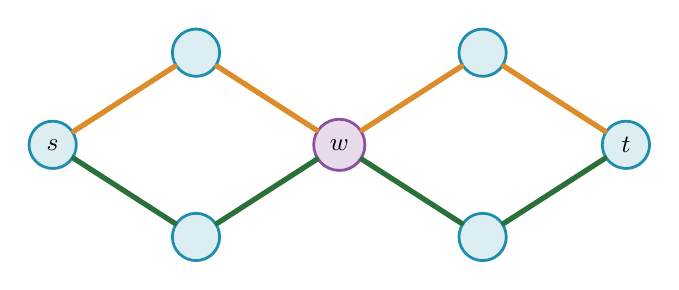
\begin{tikzpicture}[>=Stealth, scale=1.3,
    mv/.style={gvertex},
    cut/.style={gvcut, minimum size=6.5mm},
    pA/.style={grA, line width=1.9pt},
    pB/.style={grB, line width=1.9pt}]
  \node[mv]  (s) at (0,0)      {$s$};
  \node[mv]  (a) at (1.4,0.9)  {};
  \node[mv]  (c) at (1.4,-0.9) {};
  \node[cut] (w) at (2.8,0)    {$w$};
  \node[mv]  (b) at (4.2,0.9)  {};
  \node[mv]  (d) at (4.2,-0.9) {};
  \node[mv]  (t) at (5.6,0)    {$t$};
  \draw[pA] (s)--(a)--(w)--(b)--(t);
  \draw[pB] (s)--(c)--(w)--(d)--(t);
\end{tikzpicture}}{%
Two edge-disjoint $s$--$t$ routes both pass through $w$, so $\lec(s,t)=2$ but $\kap(s,t)=1$.}

% ============================================================================
%  tab:notation
% ============================================================================
\begin{frame}{Notation for the extremal functions}
\centering
\renewcommand{\arraystretch}{1.3}
\resizebox{\textwidth}{!}{%
\begin{tabular}{l|c|c}
\toprule
Model & edge-disjoint routes & internally vertex-disjoint routes \\
\midrule
Simple graph & $\ell_m(n)$ & $k_m(n)$ \\
Multigraph & $L_m(n)$ & $K_m(n)$ \\
$r$-uniform simple hypergraph & $\ell_m^{(r)}(n)$ & $k_m^{(r)}(n)$ \\
$r$-uniform multihypergraph & $L_m^{(r)}(n)$ & $K_m^{(r)}(n)$ \\
Simple digraph & $\ell_m^{\mathrm{dir}}(n)$ & $k_m^{\mathrm{dir}}(n)$ \\
Directed multigraph & $L_m^{\mathrm{dir}}(n)$ & $K_m^{\mathrm{dir}}(n)$ \\
Directed $r$-uniform simple hypergraph & $\ell_m^{\mathrm{dir}\,(r)}(n)$ & $k_m^{\mathrm{dir}\,(r)}(n)$ \\
Directed $r$-uniform multihypergraph & $L_m^{\mathrm{dir}\,(r)}(n)$ & $K_m^{\mathrm{dir}\,(r)}(n)$ \\
\bottomrule
\end{tabular}}
\end{frame}

% ============================================================================
%  thm:multigraph-edge + thm:leonard, merged: both are one-line undirected
%  bounds and neither carries the AI medal (the multigraph value is the
%  author's own Gomory-Hu double count, Leonard is a cited classical result)
% ============================================================================
\begin{frame}{Undirected bounds: multigraphs and Leonard}
\vfill
\begin{theorem}
For undirected multigraphs on $n$ vertices, $L_m(n) = (m-1)(n-1)$.
\end{theorem}
\vspace{12pt}
\begin{theorem}[B\'artfai, Bollob\'as, Leonard]
For all $n \ge m$ and $m \le 4$,
\[
    k_m(n) = \ell_m(n) = \floorfrac{m(n-1)}{2}.
\]
\end{theorem}
\vfill
\end{frame}

% ============================================================================
%  fig:divergence
% ============================================================================
\figframe{Edge and vertex diverge}{edge_vertex_divergence.png}{%
The edge and vertex extremal functions for $m = 2, 3, 4$ (blue shades, single curve per $m$ since they agree) and $m = 5$ (dashed blue for edge, solid orange for vertex). The vertex function diverges from the edge function at $n = 14$ and grows faster thereafter.}

% ============================================================================
%  thm:dir-arc-m2-exact + thm:dir-vertex-m2-exact, merged
% ============================================================================
\begin{frame}{Directed values at $m=2$}
\vfill
\begin{theorem}[Directed arc value at $m = 2$,\aimedal]
For simple digraphs,
\[
    \ell_2^{\mathrm{dir}}(n) = \max\!\left(2(n-1),\ \floorfrac{n^2}{4}\right).
\]
\end{theorem}
\vspace{12pt}
\begin{theorem}[Directed vertex value at $m = 2$,\aimedal]
For simple digraphs, $k_2^{\mathrm{dir}}(n) = \ell_2^{\mathrm{dir}}(n)$.
\end{theorem}
\vfill
\end{frame}

% ============================================================================
%  prop:hyper-edge
% ============================================================================
\begin{frame}{Hypergraph edge bound}
\vfill
\begin{proposition}[Hypergraph edge bound,\aimedal]
An $r$-uniform multihypergraph on $n$ vertices with Berge edge-connectivity at most $m-1$ has total hyperedge multiplicity at most $\floorfrac{(m-1)(n-1)}{r-1}$. A simple hypergraph attains the bound whenever $m - 1 \le \binom{n-2}{r-2}$, and a multihypergraph attains it whenever $(r-1) \mid n - 1$.
\end{proposition}
\vfill
\end{frame}

% ============================================================================
%  fig:simple-digraph-m2
% ============================================================================
\tikzframe{The two branches tie at $n=7$}{%
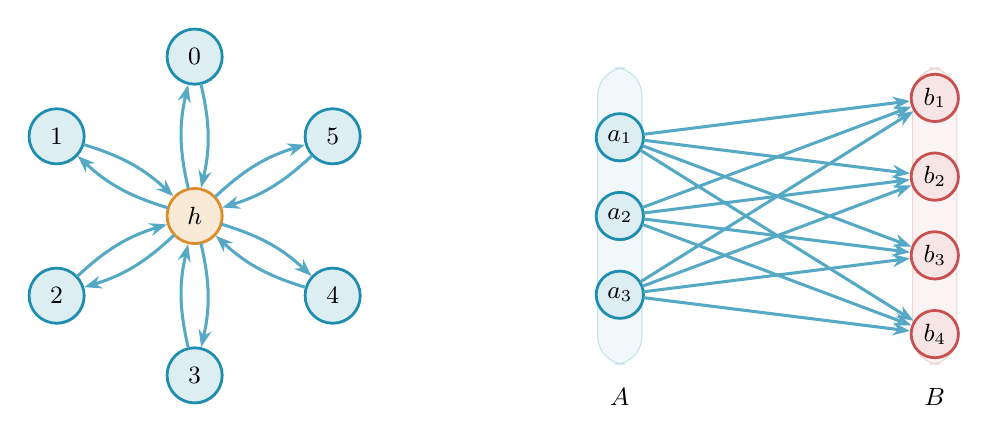
\begin{tikzpicture}[>=Stealth, scale=1.0,
    smallleftvertex/.style={gvertex}, smallrightvertex/.style={gvsink},
    hubvertex/.style={gvhub}, leftvertex/.style={gvertex},
    arc/.style={gdir},
    carc/.style={gdir, vertexorange!80!black}]
  \begin{scope}[shift={(-5.4,1.0)}, scale=0.92]
    \node[hubvertex, minimum size=7mm] (h) at (0,0) {$h$};
    \foreach \i/\ang in {0/90, 1/150, 2/210, 3/270, 4/330, 5/30} {
      \node[leftvertex, minimum size=7mm] (v\i) at (\ang:2.2) {$\i$};
    }
    \foreach \i in {0,...,5} {
      \draw[arc] (h) to[bend left=13] (v\i);
      \draw[arc] (v\i) to[bend left=13] (h);
    }
  \end{scope}
  \begin{scope}[on background layer]
    \node[draw=KULblauw1!25, fill=KULblauw1!6, rounded corners=10pt,
          fit={(0,-0.6) (0,2.6)}, inner sep=8pt, minimum width=12pt] {};
    \node[draw=vertexred!25, fill=vertexred!6, rounded corners=10pt,
          fit={(4,-0.6) (4,2.6)}, inner sep=8pt, minimum width=12pt] {};
  \end{scope}
  \foreach \i in {1,...,3} {
    \node[smallleftvertex]  (a\i) at (0, {2.0-1.0*(\i-1)}) {$a_{\i}$};
  }
  \foreach \j in {1,...,4} {
    \node[smallrightvertex] (b\j) at (4, {2.5-1.0*(\j-1)}) {$b_{\j}$};
  }
  \foreach \i in {1,...,3} {
    \foreach \j in {1,...,4} {
      \draw[arc] (a\i) -- (b\j);
    }
  }
  \node[font=\small] at (0,-1.3) {$A$};
  \node[font=\small] at (4,-1.3) {$B$};
\end{tikzpicture}}{%
The two branches tie at $n=7$, where each holds $12$ arcs at $\lec^{\max}=1$. Left: the bidirected star, a hub joined to six spokes both ways, $2(n-1)=12$. Right: the one-directional complete bipartite digraph $B_{3,4}$, every arc from $A$ to $B$, $\floor{n^2/4}=12$.}

% ============================================================================
%  thm:hyper-vertex-m2
% ============================================================================
\begin{frame}{Hypergraph vertices at $m=2$}
\vfill
\begin{theorem}[Hypergraph vertex value at $m = 2$,\aimedal]
For $r \ge 2$ and $n \ge 1$, the maximum number of hyperedges of an
$r$-uniform multihypergraph on $n$ vertices with $\kap^{\max} \le 1$ is
\[
    K_2^{(r)}(n) \;=\; \floorfrac{n-1}{r-1},
\]
attained by the star hypertree, which is simple. In
particular $K_2^{(r)}(n) = k_2^{(r)}(n) = \ell_2^{(r)}(n)$: the vertex and edge
problems agree at $m = 2$ for every uniformity, and repeated hyperedges never
help.
\end{theorem}
\vfill
\end{frame}

% ============================================================================
%  thm:hyper-vertex-m3
% ============================================================================
\begin{frame}{Hypergraph vertices at $m=3$}
\vfill
\begin{theorem}[Hypergraph vertex value at $m = 3$,\aimedal]
For $r \ge 2$, every $r$-uniform multihypergraph on $n$ vertices with
$\kap^{\max} \le 2$ has at most $\floorfrac{2(n-1)}{r-1}$ hyperedges. For
$r \ge 3$ with $2 \le \binom{n-2}{r-2}$ the bound is attained by a simple
hypergraph, so
\[
    k_3^{(r)}(n) \;=\; \floorfrac{2(n-1)}{r-1} \;=\; \ell_3^{(r)}(n).
\]
A multihypergraph attains it whenever $(r-1) \mid (n-1)$ instead, by repeating one
hyperedge rather than needing $\binom{n-2}{r-2}$ distinct ones, so
$K_3^{(r)}(n)$ takes the same value on that range.
\end{theorem}
\vfill
\end{frame}

% ============================================================================
%  thm:dir-arc-linear-error + thm:dir-vertex-linear-error, merged: the two
%  hypotheses (lambda vs kappa) drive the SAME inequality, stated once
% ============================================================================
\begin{frame}{The quadratic bound: directed arcs and vertices}
\small
\vfill
\begin{theorem}[The quadratic bound with a linear error,\aimedal]
For all $m \ge 2$ and $n \ge 2$, every simple digraph $D$ on $n$ vertices with $\lec^{\max}_D \le m-1$ satisfies
\[
    |A(D)| \;\le\; \floorfrac{n^2}{4} \;+\; 4(m-1)(n-1),
\]
so for each fixed $m$,
\[
    \ell_m^{\mathrm{dir}}(n) \;=\; \frac{n^2}{4} \;+\; \Theta_m(n) \qquad (m\ge3),
\]
and, for $m\ge3$, both the leading constant $\tfrac14$ and the order of the second-order term hold unconditionally. At $m=2$, $\ell_2^{\mathrm{dir}}(n)=n^2/4+O(1)$ as $n\to\infty$.
\end{theorem}
\vspace{8pt}
\begin{theorem}[Directed vertex problem, leading constant and order,\aimedal]
The same bound holds under the weaker hypothesis $\kap^{\max}_D \le m-1$, and consequently, for each fixed $m$,
\[
    k_m^{\mathrm{dir}}(n) \;=\; \frac{n^2}{4} \;+\; \Theta_m(n) \qquad (m\ge3).
\]
\end{theorem}
\vfill
\end{frame}

% ============================================================================
%  thm:dir-multi-full
% ============================================================================
\begin{frame}{Directed multigraphs, closed}
\vfill
\begin{theorem}[Directed multigraph value, every $n$ and $m$,\aimedal]
For all $n \ge 2$ and $m \ge 2$,
\[
    L_m^{\mathrm{dir}}(n) \;=\; (m-1)\,M(n), \qquad M(n) := \max\!\Bigl(2(n-1),\ \floorfrac{n^2}{4}\Bigr).
\]
\end{theorem}
\vfill
\end{frame}

% ============================================================================
%  thm:dir-hyper-constant
% ============================================================================
\begin{frame}{The directed hypergraph constant}
\vfill
\begin{theorem}[The directed hypergraph constant,\aimedal]
Let $r \ge 2$ and $m \ge 2$. Every forward directed $r$-uniform multihypergraph
$\HH$ on $n \ge 2$ vertices with $\kap^{\max}_{\HH} \le m-1$ satisfies
\[
    |E(\HH)| \;\le\; \frac{m-1}{r-1}\floorfrac{n^2}{4} \;+\; 4(m-1)^2 (n-1).
\]
The same bound therefore holds under $\lec^{\max}_{\HH} \le m-1$, which is the
stronger hypothesis by $\kap \le \lec$. Hence for fixed $r$ and $m$ both the
edge- and the vertex-disjoint maxima are
$\bigl(1+o(1)\bigr)(m-1)n^2/\bigl(4(r-1)\bigr)$, and the bipartite construction
is asymptotically optimal for both.
\end{theorem}
\vfill
\end{frame}

% ============================================================================
%  fig:spine
% ============================================================================
\tikzframe{The architecture}{%
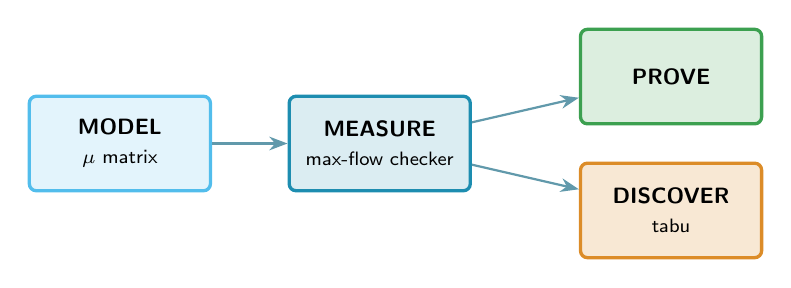
\begin{tikzpicture}[>=Stealth,
  rolenode/.style={rounded corners=2.5pt, draw, very thick, align=center,
     minimum width=23mm, minimum height=12mm, font=\sffamily\footnotesize},
  flow/.style={->, thick, KULblauw3b!70}]
  \node[rolenode, fill=roleModel!16,    draw=roleModel]    (mod) at (0,0)     {\textbf{MODEL}\\[1pt]\scriptsize $\mu$ matrix};
  \node[rolenode, fill=roleMeasure!16,  draw=roleMeasure]  (mea) at (3.3,0)   {\textbf{MEASURE}\\[1pt]\scriptsize max-flow checker};
  \node[rolenode, fill=roleProve!18,    draw=roleProve]    (pro) at (7.0,0.85){\textbf{PROVE}};
  \node[rolenode, fill=roleDiscover!20, draw=roleDiscover] (dis) at (7.0,-0.85){\textbf{DISCOVER}\\[1pt]\scriptsize tabu};
  \draw[flow] (mod) -- (mea);
  \draw[flow] (mea) -- (pro);
  \draw[flow] (mea) -- (dis);
\end{tikzpicture}}{}

% ============================================================================
%  fig:checker-gadgets  (three subfigures side by side)
% ============================================================================
\begin{frame}{Transformations}
\centering
\resizebox{\linewidth}{!}{%
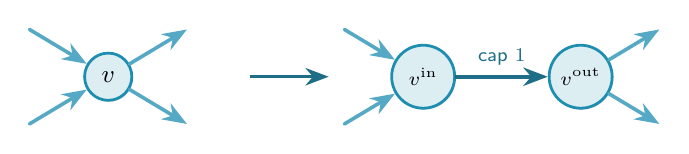
\begin{tikzpicture}[>=Stealth]
\node[vertex] (v) at (1.0, 0) {$v$};
\draw[->, edge] (0.0,  0.6) -- (v);
\draw[->, edge] (0.0, -0.6) -- (v);
\draw[->, edge] (v) -- (2.0,  0.6);
\draw[->, edge] (v) -- (2.0, -0.6);
\draw[->, very thick, color=KULblauw3b] (2.8, 0) -- (3.8, 0);
\node[smallvertex, minimum size=8mm] (vi) at (5.0, 0) {$v^{\mathrm{in}}$};
\node[smallvertex, minimum size=8mm] (vo) at (7.0, 0) {$v^{\mathrm{out}}$};
\draw[->, edge, color=KULblauw3b] (vi) -- node[above, font=\scriptsize]{cap $1$} (vo);
\draw[->, edge] (4.0,  0.6) -- (vi);
\draw[->, edge] (4.0, -0.6) -- (vi);
\draw[->, edge] (vo) -- (8.0,  0.6);
\draw[->, edge] (vo) -- (8.0, -0.6);
\end{tikzpicture}}%
\end{frame}


\begin{frame}{Transformations}
\centering
\resizebox{\linewidth}{!}{%
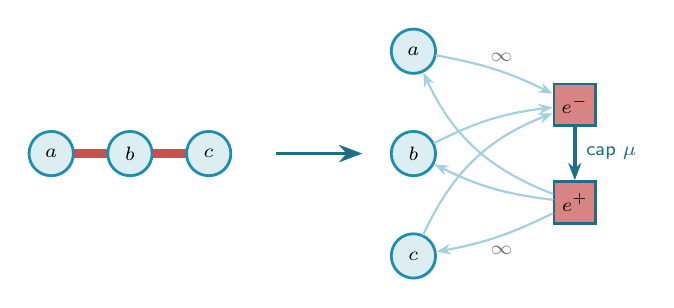
\begin{tikzpicture}[>=Stealth]
\coordinate (a) at (0.0, 0.0); \coordinate (b) at (1.0, 0.0); \coordinate (c) at (2.0, 0.0);
\begin{scope}[on background layer]\draw[metro, metroA] (a)--(b)--(c);\end{scope}
\node[smallvertex] at (a) {$a$}; \node[smallvertex] at (b) {$b$}; \node[smallvertex] at (c) {$c$};
\draw[->, very thick, color=KULblauw3b] (2.85, 0.0) -- (3.95, 0.0);
\begin{scope}[xshift=4.6cm]
\node[smallvertex] (a2) at (0.0,  1.30) {$a$};
\node[smallvertex] (b2) at (0.0,  0.00) {$b$};
\node[smallvertex] (c2) at (0.0, -1.30) {$c$};
\node[hnode, fill=metroA!70, minimum size=15pt] (em) at (2.05,  0.62) {$e^-$};
\node[hnode, fill=metroA!70, minimum size=15pt] (ep) at (2.05, -0.62) {$e^+$};
\draw[gdirfaint] (a2) to[bend left=8]  node[above, font=\scriptsize, text=black!55, pos=0.55]{$\infty$} (em);
\draw[gdirfaint] (b2) to[bend left=10] (em);
\draw[gdirfaint] (c2) to[bend left=22] (em);
\draw[gdirfaint] (ep) to[bend left=22] (a2);
\draw[gdirfaint] (ep) to[bend left=10] (b2);
\draw[gdirfaint] (ep) to[bend left=8]  node[below, font=\scriptsize, text=black!55, pos=0.45]{$\infty$} (c2);
\draw[gdir, line width=1.6pt, color=KULblauw3b] (em) -- node[right, font=\scriptsize]{cap $\mu$} (ep);
\end{scope}
\end{tikzpicture}}
\end{frame}


\begin{frame}{Transformations}
\centering
\resizebox{\linewidth}{!}{%
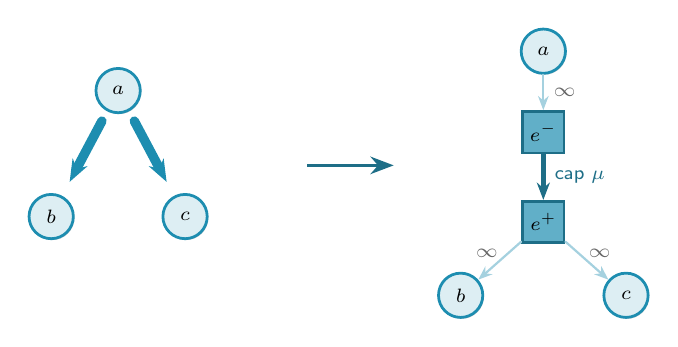
\begin{tikzpicture}[>=Stealth, gatearc/.style={gdir}]
\node[smallvertex] (a) at (0.0, 1.05) {$a$}; \node[smallvertex] (b) at (-0.85, -0.55) {$b$}; \node[smallvertex] (c) at (0.85, -0.55) {$c$};
\begin{scope}[on background layer]
  \draw[metro, metroB, -{Stealth[length=2.8mm]}, shorten >=2mm, shorten <=1.4mm] (a) -- (b);
  \draw[metro, metroB, -{Stealth[length=2.8mm]}, shorten >=2mm, shorten <=1.4mm] (a) -- (c);
\end{scope}
\draw[->, very thick, color=KULblauw3b] (2.4, 0.1) -- (3.5, 0.1);
\begin{scope}[xshift=5.4cm]
  \node[smallvertex] (a2) at (0.0, 1.55) {$a$};
  \node[hnode, fill=metroB!70, minimum size=15pt] (gm) at (0.0,  0.52) {$e^-$};
  \node[hnode, fill=metroB!70, minimum size=15pt] (gp) at (0.0, -0.62) {$e^+$};
  \node[smallvertex] (b2) at (-1.05, -1.55) {$b$}; \node[smallvertex] (c2) at (1.05, -1.55) {$c$};
  \draw[gdirfaint] (a2) -- node[right, font=\scriptsize, text=black!60]{$\infty$} (gm);
  \draw[gdir, line width=1.6pt, color=KULblauw3b] (gm) -- node[right, font=\scriptsize]{cap $\mu$} (gp);
  \draw[gdirfaint] (gp) -- node[left, pos = 0.3, font=\scriptsize, text=black!60]{$\infty$} (b2);
  \draw[gdirfaint] (gp) -- node[right, pos = 0.3, font=\scriptsize, text=black!60]{$\infty$} (c2);
\end{scope}
\end{tikzpicture}}
\end{frame}

% ============================================================================
%  fig:complexity
% ============================================================================
\figframe{Candidate counts}{complexity_growth.png}{}

% ============================================================================
%  fig:matrix-rep
% ============================================================================
\tikzframescaled{The two encodings}{%
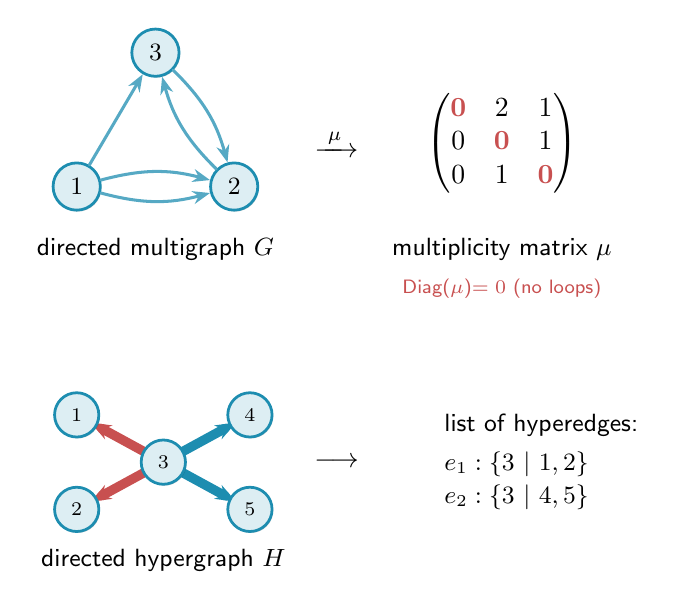
\begin{tikzpicture}[>=Stealth]
\node[vertex] (A) at (0,   0)   {$1$};
\node[vertex] (B) at (2.0, 0)   {$2$};
\node[vertex] (C) at (1.0, 1.7) {$3$};
\draw[arc] (A) to[bend left=15]  (B);
\draw[arc] (A) to[bend right=15] (B);
\draw[arc] (B) to[bend left=15]  (C);
\draw[arc] (C) to[bend left=15] (B);
\draw[arc] (A) -- (C);
\node[font=\small] at (1.0, -0.8) {directed multigraph $G$};
\node at (3.3, 0.55) {$\xrightarrow{\;\mu\;}$};
\node at (5.4, 0.55) {$\begin{pmatrix} {\color{vertexred}\mathbf 0} & 2 & 1 \\ 0 & {\color{vertexred}\mathbf 0} & 1 \\ 0 & 1 & {\color{vertexred}\mathbf 0} \end{pmatrix}$};
\node[font=\small] at (5.4, -0.8) {multiplicity matrix $\mu$};
\node[font=\scriptsize, vertexred] at (5.4, -1.3) {Diag($\mu$)$=0$ (no loops)};
\begin{scope}[yshift=-3.5cm]
  \coordinate (p1) at (0.0, 0.6);
  \coordinate (p2) at (0.0,-0.6);
  \coordinate (p3) at (1.1, 0.0);
  \coordinate (p4) at (2.2, 0.6);
  \coordinate (p5) at (2.2,-0.6);
  \begin{scope}[on background layer]
    \draw[metro, metroA, -{Stealth[length=2.6mm]}, shorten >=2mm, shorten <=1.4mm] (p3) -- (p1);
    \draw[metro, metroA, -{Stealth[length=2.6mm]}, shorten >=2mm, shorten <=1.4mm] (p3) -- (p2);
    \draw[metro, metroB, -{Stealth[length=2.6mm]}, shorten >=2mm, shorten <=1.4mm] (p3) -- (p4);
    \draw[metro, metroB, -{Stealth[length=2.6mm]}, shorten >=2mm, shorten <=1.4mm] (p3) -- (p5);
  \end{scope}
  \foreach \p/\lbl in {p1/1,p2/2,p3/3,p4/4,p5/5} {\node[smallvertex] at (\p) {$\lbl$};}
  \node[font=\small] at (1.1,-1.25) {directed hypergraph $H$};
  \node at (3.3, 0.0) {$\longrightarrow$};
  \node[font=\small, align=left] at (5.9, 0.0)
    {list of hyperedges:\\[3pt] $e_1: \{3\ |\ 1,2\}$\\[1pt] $e_2:\{3\ |\ 4,5\}$};
\end{scope}
\end{tikzpicture}}{%
The two encodings, for the directed variants. The digraph is the multiplicity matrix $\mu$, where $\mu_{ij}$ counts arcs from $i$ to $j$. The directed hypergraph is a list of hyperedges, with the tail of each isolated. Multihypergraphs repeat at least one entry in the list.}{0.72}

% ============================================================================
%  fig:prune
% ============================================================================
\tikzframe{Branch and bound}{%
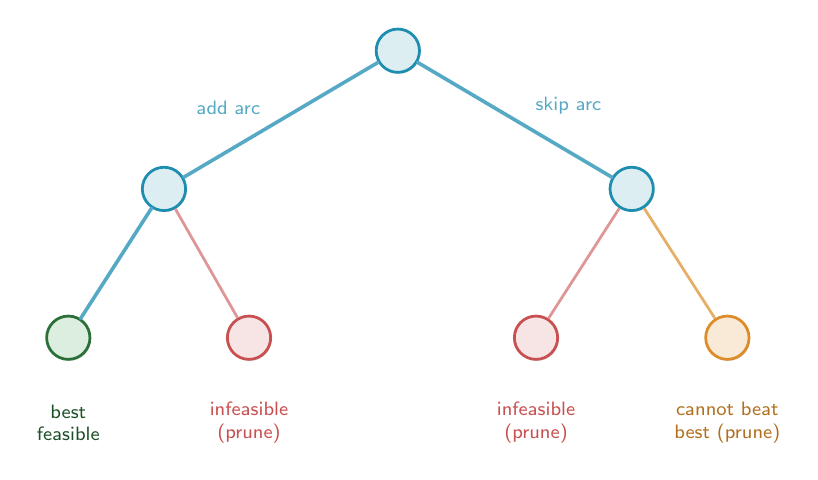
\begin{tikzpicture}[scale=1.35, >=Stealth,
   live/.style={gvertex, minimum size=5.5mm},
   dead/.style={gvsink, minimum size=5.5mm},
   bnd/.style={gvhub, minimum size=5.5mm},
   best/.style={gvertex, draw=vertexgreen!70!black, fill=vertexgreen!18, minimum size=5.5mm},
   br/.style={gline}]
  \node[live] (r) at (0,0) {};
  \node[live] (l) at (-2.2,-1.3) {};
  \node[live] (rr) at (2.2,-1.3) {};
  \draw[br] (r) -- node[above left, font=\scriptsize, pos=0.55]{add arc} (l);
  \draw[br] (r) -- node[above right, font=\scriptsize, pos=0.55]{skip arc} (rr);
  \node[best] (l1) at (-3.1,-2.7) {};
  \node[dead] (l2) at (-1.4,-2.7) {};
  \draw[br] (l)--(l1);
  \draw[line width=1pt, vertexred!60] (l)--(l2);
  \node[dead] (r1) at (1.3,-2.7) {};
  \node[bnd]  (r2) at (3.1,-2.7) {};
  \draw[line width=1pt, vertexred!60] (rr)--(r1);
  \draw[line width=1pt, vertexorange!70] (rr)--(r2);
  \node[font=\scriptsize, vertexgreen!50!black, align=center] at (-3.1,-3.5) {best\\feasible};
  \node[font=\scriptsize, vertexred, align=center] at (-1.4,-3.5) {infeasible\\(prune)};
  \node[font=\scriptsize, vertexred, align=center] at (1.3,-3.5) {infeasible\\(prune)};
  \node[font=\scriptsize, vertexorange!80!black, align=center] at (3.1,-3.5) {cannot beat\\best (prune)};
\end{tikzpicture}}{%
Each level of the partially built graph fixes one adjacency. Infeasible partial graphs (red) and branches unable to beat the incumbent (orange) are discarded.}

% ============================================================================
%  generating-search benchmark table
% ============================================================================
\begin{frame}{Generating search: a benchmark}
\centering
\renewcommand{\arraystretch}{1.2}
\begin{tabular}{rrrrr}
\toprule
$n$ & $\ell_2^{\mathrm{dir}}(n)$ & blind (s) & pruned (s) & generated (s) \\
\midrule
3 & 4  & 0.05 & 0.003 & 0.009 \\
4 & 6  & 6.3  & 0.008 & 0.008 \\
5 & 8  & --   & 0.22  & 0.039 \\
6 & 10 & --   & 14.5  & 0.73  \\
7 & 12 & --   & 1156.6 & 17.0 \\
\bottomrule
\end{tabular}
\end{frame}

% ============================================================================
%  fig:scaling-reduction
% ============================================================================
\tikzframe{Scaling out $m$}{%
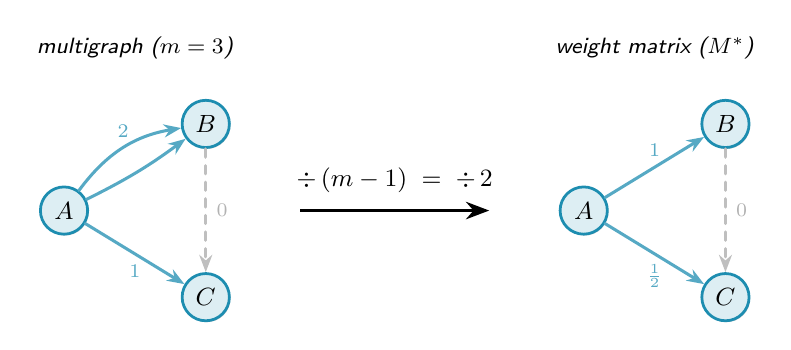
\begin{tikzpicture}[>=Stealth, font=\small]
    \node[vertex] (A1) at (-4.2, 0)   {$A$};
    \node[vertex] (B1) at (-2.4, 1.1) {$B$};
    \node[vertex] (C1) at (-2.4,-1.1) {$C$};
    \draw[->, arc] (A1) to[bend left=22]  node[above, font=\scriptsize]{$2$} (B1);
    \draw[->, arc] (A1) to[bend right=5]  (B1);
    \draw[->, arc] (A1) -- node[below, font=\scriptsize]{$1$} (C1);
    \draw[->, arc, color=gray!50, dashed] (B1) -- node[right, font=\scriptsize, color=gray!60]{$0$} (C1);
    \node[above, font=\footnotesize\itshape] at (-3.3, 1.8) {multigraph ($m=3$)};
    \draw[->, very thick] (-1.2, 0) -- (1.2, 0);
    \node[above, font=\small] at (0, 0.1) {$\div\,(m-1)\;=\;\div\,2$};
    \node[vertex] (A2) at (2.4, 0)   {$A$};
    \node[vertex] (B2) at (4.2, 1.1) {$B$};
    \node[vertex] (C2) at (4.2,-1.1) {$C$};
    \draw[->, arc] (A2) -- node[above, font=\scriptsize]{$1$} (B2);
    \draw[->, arc] (A2) -- node[below, font=\scriptsize]{$\tfrac{1}{2}$} (C2);
    \draw[->, arc, color=gray!50, dashed] (B2) -- node[right, font=\scriptsize, color=gray!60]{$0$} (C2);
    \node[above, font=\footnotesize\itshape] at (3.3, 1.8) {weight matrix ($M^*$)};
\end{tikzpicture}}{%
Scaling at $m=3$: dividing multiplicities by $m-1=2$ turns the integer multigraph into a weight matrix with entries in $[0,1]$ and pairwise maximum flow at most one. Hence one $m$-free optimisation bounds every threshold.}

% ============================================================================
%  energy function
% ============================================================================
\begin{frame}{The search: an energy function}
\vfill
To implement the metaheuristic, give each graph one number: its energy
\[
    \Phi(G) = -|E(G)| + \Lambda \cdot \max\bigl(0,\ c^{\max}(G) - (m - 1)\bigr).
\]
\vfill
\end{frame}

% ============================================================================
%  what the search rediscovers (table)
% ============================================================================
\begin{frame}{What the search rediscovers}
\centering
\scriptsize
\renewcommand{\arraystretch}{1.25}
\begin{tabular}{llccrr}
\toprule
Construction & Variant & $n$ & $m$ & Search & Theory \\
\midrule
spanning tree (simple undirected) & $\ell_m(n)$ & 6 & 2 & 5 & 5 \\
multiplicity-$(m{-}1)$ star (multi undirected) & $L_m(n)$ & 6 & 3 & 10 & 10 \\
bidirected star (simple directed) & $\ell_m^{\mathrm{dir}}(n)$ & 4 & 2 & 6 & 6 \\
bidirected star (simple directed) & $\ell_m^{\mathrm{dir}}(n)$ & 6 & 2 & 10 & 10 \\
hub--bipartite tie (simple directed) & $\ell_m^{\mathrm{dir}}(n)$ & 7 & 2 & 12 & 12 \\
double star (multi directed) & $L_m^{\mathrm{dir}}(n)$ & 4 & 3 & 12 & 12 \\
double star (multi directed) & $L_m^{\mathrm{dir}}(n)$ & 5 & 3 & 16 & 16 \\
\bottomrule
\end{tabular}
\end{frame}

% ============================================================================
%  fig:rediscovery-gallery
% ============================================================================
\tikzframescaled{Three rediscovered shapes}{%
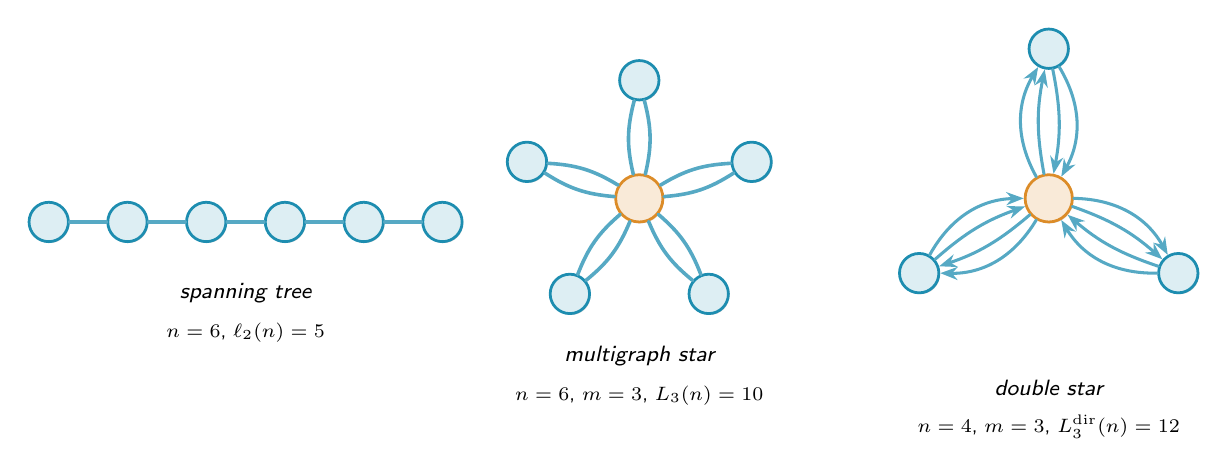
\begin{tikzpicture}[>=Stealth]
  \begin{scope}[shift={(-7.5,0)}]
    \foreach \i/\x in {1/0,2/1.0,3/2.0,4/3.0,5/4.0,6/5.0} {
      \node[gvertex, minimum size=5mm] (t\i) at (\x,0) {};
    }
    \foreach \i/\j in {1/2,2/3,3/4,4/5,5/6} {
      \draw[gline] (t\i) -- (t\j);
    }
    \node[font=\footnotesize\itshape] at (2.5,-0.9) {spanning tree};
    \node[font=\scriptsize] at (2.5,-1.4) {$n=6$, $\ell_2(n)=5$};
  \end{scope}
  \begin{scope}[shift={(0,0.3)}]
    \node[gvhub, minimum size=6mm] (h2) at (0,0) {};
    \foreach \ang in {90,162,234,306,18} {
      \node[gvertex, minimum size=5mm] (l2\ang) at (\ang:1.5) {};
      \draw[gline] (h2) to[gcurve]  (l2\ang);
      \draw[gline] (h2) to[gcurveR] (l2\ang);
    }
    \node[font=\footnotesize\itshape] at (0,-2.0) {multigraph star};
    \node[font=\scriptsize] at (0,-2.5) {$n=6$, $m=3$, $L_3(n)=10$};
  \end{scope}
  \begin{scope}[shift={(5.2,0.3)}]
    \node[gvhub, minimum size=6mm] (h3) at (0,0) {};
    \foreach \ang in {90,210,330} {
      \node[gvertex, minimum size=5mm] (l3\ang) at (\ang:1.9) {};
      \draw[gdir] (h3)     to[bend left=30]  (l3\ang);
      \draw[gdir] (h3)     to[bend left=11]  (l3\ang);
      \draw[gdir] (l3\ang) to[bend left=30]  (h3);
      \draw[gdir] (l3\ang) to[bend left=11]  (h3);
    }
    \node[font=\footnotesize\itshape] at (0,-2.4) {double star};
    \node[font=\scriptsize] at (0,-2.9) {$n=4$, $m=3$, $L_3^{\mathrm{dir}}(n)=12$};
  \end{scope}
\end{tikzpicture}}{%
Three of the shapes the search rediscovers, each drawn at the size the table reports. The fourth, the bidirected star tying the one-directional wall at $n=7$, was shown earlier.}{0.95}

% ============================================================================
%  fig:crossover
% ============================================================================
\figframe{The directed crossover}{directed_crossover.png}{%
The two lower-bound branches of the directed-arc conjecture at $m = 3$, and the maximum they define.}

% ============================================================================
%  fig:augmented-wall
% ============================================================================
\tikzframe{The augmented bipartite digraph}{%
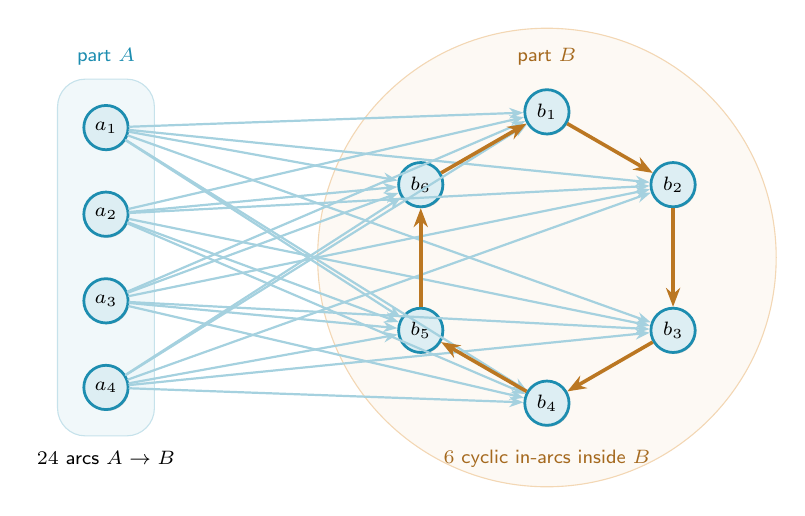
\begin{tikzpicture}[>=Stealth, scale=1.0,
    wallarc/.style={gdirfaint},
    cyc/.style={-{Stealth[length=2.4mm]}, line width=1.3pt, vertexorange!85!black}]
  \foreach \i/\y in {1/1.65, 2/0.55, 3/-0.55, 4/-1.65} {
    \node[smallvertex] (a\i) at (0,\y) {$a_{\i}$};
  }
  \foreach \j/\ang in {1/90, 2/30, 3/-30, 4/-90, 5/-150, 6/150} {
    \node[smallvertex] (b\j) at ($(5.6,0)+(\ang:1.85)$) {$b_{\j}$};
  }
  \begin{scope}[on background layer]
    \node[draw=KULblauw1!25, fill=KULblauw1!6, rounded corners=10pt,
          fit={(a1) (a4)}, inner sep=9pt] {};
    \node[draw=vertexorange!35, fill=vertexorange!5, circle,
          fit={(b1) (b2) (b3) (b4) (b5) (b6)}, inner sep=1pt] {};
  \end{scope}
  \node[font=\scriptsize, KULblauw1] at (0,2.55) {part $A$};
  \node[font=\scriptsize, vertexorange!75!black] at (5.6,2.55) {part $B$};
  \foreach \i in {1,...,4}{\foreach \j in {1,...,6}{\draw[wallarc] (a\i) -- (b\j);}}
  \foreach \j/\k in {1/2, 2/3, 3/4, 4/5, 5/6, 6/1} {
    \draw[cyc] (b\j) -- (b\k);
  }
  \node[font=\scriptsize] at (0,-2.55) {$24$ arcs $A \to B$};
  \node[font=\scriptsize, align=center, vertexorange!75!black] at (5.6,-2.55)
    {$6$ cyclic in-arcs inside $B$};
\end{tikzpicture}}{%
The augmented bipartite digraph at $m = 3$, $n = 10$. Every cross-part arc runs from $A$ to $B$, and inside $B$ each vertex takes one arc from its cyclic predecessor, which is $m - 2$ arcs per vertex. A pair $a_i, b_j$ then has the direct arc and one detour, so $\lec^{\max} = 2$, and the count is $24 + 6 = 30$ against the hub branch's $27$.}

% ============================================================================
%  fig:variant-tree-status
% ============================================================================
\begin{frame}{Status of the sixteen variants}
\vspace{-4pt}
\begin{center}
\adjustbox{max totalheight=0.62\textheight}{\resizebox{\textwidth}{!}{%
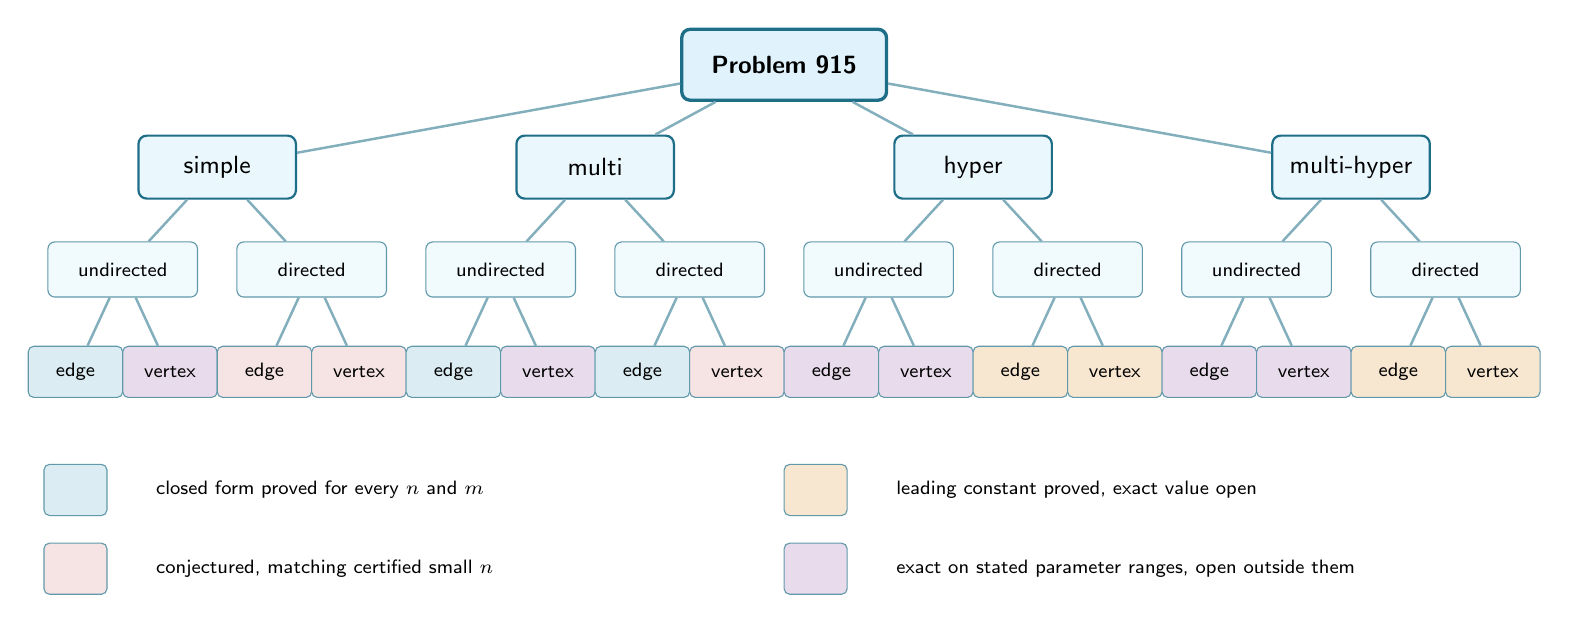
\begin{tikzpicture}
  \node[vtroot, fill=KULblauw3a!18]  (root) at (9.0,3.9) {Problem 915};
  \node[vtmodel, fill=KULblauw3a!12] (simple) at (1.8,2.6)  {simple};
  \node[vtmodel, fill=KULblauw3a!12] (multi)  at (6.6,2.6)  {multi};
  \node[vtmodel, fill=KULblauw3a!12] (hyper)  at (11.4,2.6) {hyper};
  \node[vtmodel, fill=KULblauw3a!12] (mhyper) at (16.2,2.6) {multi-hyper};
  \draw[vtedge] (root) -- (simple);
  \draw[vtedge] (root) -- (multi);
  \draw[vtedge] (root) -- (hyper);
  \draw[vtedge] (root) -- (mhyper);
  \node[vtdir, fill=KULblauw3a!8]  (d0) at (0.6,1.3)  {undirected};
  \node[vtdir, fill=KULblauw3a!8]  (d1) at (3.0,1.3)  {directed};
  \node[vtdir, fill=KULblauw3a!8]  (d2) at (5.4,1.3)  {undirected};
  \node[vtdir, fill=KULblauw3a!8]  (d3) at (7.8,1.3)  {directed};
  \node[vtdir, fill=KULblauw3a!8]  (d4) at (10.2,1.3) {undirected};
  \node[vtdir, fill=KULblauw3a!8]  (d5) at (12.6,1.3) {directed};
  \node[vtdir, fill=KULblauw3a!8]  (d6) at (15.0,1.3) {undirected};
  \node[vtdir, fill=KULblauw3a!8]  (d7) at (17.4,1.3) {directed};
  \draw[vtedge] (simple) -- (d0);
  \draw[vtedge] (simple) -- (d1);
  \draw[vtedge] (multi)  -- (d2);
  \draw[vtedge] (multi)  -- (d3);
  \draw[vtedge] (hyper)  -- (d4);
  \draw[vtedge] (hyper)  -- (d5);
  \draw[vtedge] (mhyper) -- (d6);
  \draw[vtedge] (mhyper) -- (d7);
  \node[vtleaf, fill=regimeProved!16]      (l0)  at (0,0)    {edge};
  \node[vtleaf, fill=regimePartial!20]     (l1)  at (1.2,0)  {vertex};
  \node[vtleaf, fill=regimeConjectured!16] (l2)  at (2.4,0)  {edge};
  \node[vtleaf, fill=regimeConjectured!16] (l3)  at (3.6,0)  {vertex};
  \node[vtleaf, fill=regimeProved!16]      (l4)  at (4.8,0)  {edge};
  \node[vtleaf, fill=regimePartial!20]     (l5)  at (6.0,0)  {vertex};
  \node[vtleaf, fill=regimeProved!16]      (l6)  at (7.2,0)  {edge};
  \node[vtleaf, fill=regimeConjectured!16] (l7)  at (8.4,0)  {vertex};
  \node[vtleaf, fill=regimePartial!20]     (l8)  at (9.6,0)  {edge};
  \node[vtleaf, fill=regimePartial!20]     (l9)  at (10.8,0) {vertex};
  \node[vtleaf, fill=regimeOpen!22]        (l10) at (12.0,0) {edge};
  \node[vtleaf, fill=regimeOpen!22]        (l11) at (13.2,0) {vertex};
  \node[vtleaf, fill=regimePartial!20]     (l12) at (14.4,0) {edge};
  \node[vtleaf, fill=regimePartial!20]     (l13) at (15.6,0) {vertex};
  \node[vtleaf, fill=regimeOpen!22]        (l14) at (16.8,0) {edge};
  \node[vtleaf, fill=regimeOpen!22]        (l15) at (18.0,0) {vertex};
  \draw[vtedge] (d0) -- (l0);  \draw[vtedge] (d0) -- (l1);
  \draw[vtedge] (d1) -- (l2);  \draw[vtedge] (d1) -- (l3);
  \draw[vtedge] (d2) -- (l4);  \draw[vtedge] (d2) -- (l5);
  \draw[vtedge] (d3) -- (l6);  \draw[vtedge] (d3) -- (l7);
  \draw[vtedge] (d4) -- (l8);  \draw[vtedge] (d4) -- (l9);
  \draw[vtedge] (d5) -- (l10); \draw[vtedge] (d5) -- (l11);
  \draw[vtedge] (d6) -- (l12); \draw[vtedge] (d6) -- (l13);
  \draw[vtedge] (d7) -- (l14); \draw[vtedge] (d7) -- (l15);
  \node[vtleaf, fill=regimeProved!16, minimum width=8mm]      (leg1) at (0,-1.5) {};
  \node[anchor=west, font=\scriptsize] at (0.9,-1.5) {closed form proved for every $n$ and $m$};
  \node[vtleaf, fill=regimeConjectured!16, minimum width=8mm] (leg2) at (0,-2.5) {};
  \node[anchor=west, font=\scriptsize] at (0.9,-2.5) {conjectured, matching certified small $n$};
  \node[vtleaf, fill=regimeOpen!22, minimum width=8mm]        (leg3) at (9.4,-1.5) {};
  \node[anchor=west, font=\scriptsize] at (10.3,-1.5) {leading constant proved, exact value open};
  \node[vtleaf, fill=regimePartial!20, minimum width=8mm]     (leg4) at (9.4,-2.5) {};
  \node[anchor=west, font=\scriptsize] at (10.3,-2.5) {exact on stated parameter ranges, open outside them};
\end{tikzpicture}}}

\end{center}

\vspace{2pt}
\noindent{\tiny\color{black!60} Status of the sixteen variants. Colour marks the status of a leaf: blue a closed form proved for every $n$ and $m$, purple an exact value proved on stated parameter ranges and open outside them, red a conjectured exact formula with a proved lower bound, and amber a proved leading term with the exact value unknown.}\par
\end{frame}

% ============================================================================
%  the four sideways variant-bounds grids
% ============================================================================
\figframetall{Eight graph variants at $m=3$}{variant_bounds_m3_graphs.png}{}

\figframetall{Eight hypergraph variants at $m=3$}{variant_bounds_m3_hypergraphs.png}{}

\figframetall{Eight graph variants at $m=6$}{variant_bounds_m6_graphs.png}{}

\figframetall{Eight hypergraph variants at $m=6$}{variant_bounds_m6_hypergraphs.png}{}

% ============================================================================
%  tab:summary
% ============================================================================
\begin{frame}{The sixteen variants, summarised}
\centering
\scriptsize
\renewcommand{\arraystretch}{1.25}
\setlength{\tabcolsep}{4pt}
\begin{tabularx}{\textwidth}{@{}>{\raggedright\arraybackslash}p{0.14\textwidth}>{\raggedright\arraybackslash}X>{\raggedright\arraybackslash}X@{}}
\toprule
Model & Edge or arc-disjoint & Vertex-disjoint \\
\midrule
\addlinespace[1pt]
\multicolumn{3}{@{}l}{\itshape Undirected} \\
\addlinespace[2pt]
simple graph
  & $\floor{m(n-1)/2}$, proved
  & the edge value for $m \le 4$, and $\floor{8n/3}-4$ at $m=5$; open for $m \ge 6$ \\
multigraph
  & $(m-1)(n-1)$, proved
  & the simple value \\
$r$-hypergraph
  & $\le \floor{(m-1)(n-1)/(r-1)}$, with equality in the range below
  & $\floor{(n-1)/(r-1)}$ at $m=2$ and $\le \floor{2(n-1)/(r-1)}$ at $m=3$; open for $m \ge 4$ \\
$r$-multi-hyper
  & the same bound, with equality when $(r-1) \mid (n-1)$
  & the same bounds, repeats closing cases the simple model misses at $m=3$ \\
\addlinespace[4pt]
\midrule
\addlinespace[1pt]
\multicolumn{3}{@{}l}{\itshape Directed} \\
\addlinespace[2pt]
simple digraph
  & $M(n)$ at $m=2$, proved; $n^2/4 + \Theta_m(n)$ for $m \ge 3$, exact value conjectured
  & $M(n)$ at $m=2$, proved; $n^2/4 + \Theta_m(n)$ for $m \ge 3$, equality with the arc value open \\
multigraph
  & $(m-1)M(n)$, proved
  & the simple digraph value \\
$r$-hypergraph
  & $(1+o(1))(m-1)n^2/[4(r-1)]$ for fixed $r, m$, leading term proved
  & the same leading term for fixed $r, m$ \\
$r$-multi-hyper
  & the same leading term, the bound proved with repeats allowed
  & the same leading term for fixed $r, m$ \\
\bottomrule
\end{tabularx}
\end{frame}

% ============================================================================
%  the exact-value tables, split at m=3 / m=6
% ============================================================================
\begin{frame}{Exact values, $m=3$}
\centering
\adjustbox{max width=\textwidth,max totalheight=0.82\textheight}{%
\begin{tabular}{llrrrrrrr}
\toprule
Model & Variant & $n=2$ & $n=3$ & $n=4$ & $n=5$ & $n=6$ & $n=7$ & $n=8$ \\
\midrule
\multirow{4}{*}{simple graph} & undirected, edge ($\ell_m(n)$), \textcolor{vtProved}{proved} & \textcolor{vtExact}{\textbf{1}} & \textcolor{vtExact}{\textbf{3}} & \textcolor{vtExact}{\textbf{4}} & \textcolor{vtExact}{\textbf{6}} & \textcolor{vtExact}{\textbf{7}} & \textcolor{vtExact}{\textbf{9}} & \textcolor{vtExact}{\textbf{10}} \\
 & undirected, vertex ($k_m(n)$), \textcolor{vtProved}{proved} & \textcolor{vtExact}{\textbf{1}} & \textcolor{vtExact}{\textbf{3}} & \textcolor{vtExact}{\textbf{4}} & \textcolor{vtExact}{\textbf{6}} & \textcolor{vtExact}{\textbf{7}} & \textcolor{vtExact}{\textbf{9}} & \textcolor{vtProved}{10} \\
 & directed, arc ($\ell_m^{\mathrm{dir}}(n)$), \textcolor{vtConjectured}{conjectured} & \textcolor{vtExact}{\textbf{2}} & \textcolor{vtExact}{\textbf{6}} & \textcolor{vtExact}{\textbf{9}} & \textcolor{vtExact}{\textbf{12}} & \textcolor{vtExact}{\textbf{15}} & \textcolor{vtConjectured}{$\ge$18} & \textcolor{vtConjectured}{$\ge$21} \\
 & directed, vertex ($k_m^{\mathrm{dir}}(n)$), \textcolor{vtConjectured}{conjectured} & \textcolor{vtExact}{\textbf{2}} & \textcolor{vtExact}{\textbf{6}} & \textcolor{vtExact}{\textbf{9}} & \textcolor{vtExact}{\textbf{12}} & \textcolor{vtExact}{\textbf{15}} & \textcolor{vtConjectured}{$\ge$18} & \textcolor{vtConjectured}{$\ge$21} \\
\midrule
\multirow{4}{*}{multigraph} & undirected, edge ($L_m(n)$), \textcolor{vtProved}{proved} & \textcolor{vtExact}{\textbf{2}} & \textcolor{vtExact}{\textbf{4}} & \textcolor{vtExact}{\textbf{6}} & \textcolor{vtExact}{\textbf{8}} & \textcolor{vtExact}{\textbf{10}} & \textcolor{vtProved}{12} & \textcolor{vtProved}{14} \\
 & undirected, vertex ($k_m(n)$), \textcolor{vtProved}{= simple, proved} & \textcolor{vtExact}{\textbf{1}} & \textcolor{vtExact}{\textbf{3}} & \textcolor{vtExact}{\textbf{4}} & \textcolor{vtExact}{\textbf{6}} & \textcolor{vtExact}{\textbf{7}} & \textcolor{vtExact}{\textbf{9}} & \textcolor{vtProved}{10} \\
 & directed, arc ($L_m^{\mathrm{dir}}(n)$), \textcolor{vtProved}{proved} & \textcolor{vtExact}{\textbf{4}} & \textcolor{vtExact}{\textbf{8}} & \textcolor{vtExact}{\textbf{12}} & \textcolor{vtExact}{\textbf{16}} & \textcolor{vtProved}{20} & \textcolor{vtProved}{24} & \textcolor{vtProved}{32} \\
 & directed, vertex ($k_m^{\mathrm{dir}}(n)$), \textcolor{vtConjectured}{= simple, conjectured} & \textcolor{vtExact}{\textbf{2}} & \textcolor{vtExact}{\textbf{6}} & \textcolor{vtExact}{\textbf{9}} & \textcolor{vtExact}{\textbf{12}} & \textcolor{vtExact}{\textbf{15}} & \textcolor{vtConjectured}{$\ge$18} & \textcolor{vtConjectured}{$\ge$21} \\
\midrule
\multirow{4}{*}{hypergraph $r=3$} & undirected, edge, \textcolor{vtProved}{proved} &  & \textcolor{vtExact}{\textbf{1}} & \textcolor{vtExact}{\textbf{3}} & \textcolor{vtExact}{\textbf{4}} & \textcolor{vtProved}{5} & \textcolor{vtProved}{6} & \textcolor{vtProved}{7} \\
 & undirected, vertex, \textcolor{vtProved}{proved} &  & \textcolor{vtExact}{\textbf{1}} & \textcolor{vtExact}{\textbf{3}} & \textcolor{vtExact}{\textbf{4}} & \textcolor{vtProved}{5} & \textcolor{vtProved}{6} & \textcolor{vtProved}{7} \\
 & directed, arc, \textcolor{vtOpen}{open} &  & \textcolor{vtExact}{\textbf{3}} & \textcolor{vtExact}{\textbf{8}} & \textcolor{vtOpen}{$\ge$10} & \textcolor{vtOpen}{$\ge$12} & \textcolor{vtOpen}{$\ge$14} & \textcolor{vtOpen}{$\ge$16} \\
 & directed, vertex, \textcolor{vtOpen}{open} &  & \textcolor{vtExact}{\textbf{3}} & \textcolor{vtExact}{\textbf{8}} & \textcolor{vtOpen}{$\ge$10} & \textcolor{vtOpen}{$\ge$12} & \textcolor{vtOpen}{$\ge$14} & \textcolor{vtOpen}{$\ge$16} \\
\midrule
\multirow{4}{*}{multihypergraph $r=3$} & undirected, edge, \textcolor{vtProved}{proved} &  & \textcolor{vtExact}{\textbf{2}} & \textcolor{vtExact}{\textbf{3}} & \textcolor{vtProved}{4} & \textcolor{vtProved}{5} & \textcolor{vtProved}{6} & \textcolor{vtProved}{7} \\
 & undirected, vertex, \textcolor{vtProved}{proved} &  & \textcolor{vtExact}{\textbf{2}} & \textcolor{vtExact}{\textbf{3}} & \textcolor{vtProved}{4} & \textcolor{vtProved}{5} & \textcolor{vtProved}{6} & \textcolor{vtProved}{7} \\
 & directed, arc, \textcolor{vtOpen}{open} &  & \textcolor{vtExact}{\textbf{6}} & \textcolor{vtOpen}{$\ge$8} & \textcolor{vtOpen}{$\ge$10} & \textcolor{vtOpen}{$\ge$12} & \textcolor{vtOpen}{$\ge$14} & \textcolor{vtOpen}{$\ge$16} \\
 & directed, vertex, \textcolor{vtOpen}{open} &  & \textcolor{vtExact}{\textbf{6}} & \textcolor{vtOpen}{$\ge$8} & \textcolor{vtOpen}{$\ge$10} & \textcolor{vtOpen}{$\ge$12} & \textcolor{vtOpen}{$\ge$14} & \textcolor{vtOpen}{$\ge$16} \\
\bottomrule
\end{tabular}}
\end{frame}

\begin{frame}{Exact values, $m=6$}
\centering
\adjustbox{max width=\textwidth,max totalheight=0.82\textheight}{%
\begin{tabular}{llrrrrrrr}
\toprule
Model & Variant & $n=2$ & $n=3$ & $n=4$ & $n=5$ & $n=6$ & $n=7$ & $n=8$ \\
\midrule
\multirow{4}{*}{simple graph} & undirected, edge ($\ell_m(n)$), \textcolor{vtProved}{proved} & \textcolor{vtExact}{\textbf{1}} & \textcolor{vtExact}{\textbf{3}} & \textcolor{vtExact}{\textbf{6}} & \textcolor{vtExact}{\textbf{10}} & \textcolor{vtExact}{\textbf{15}} & \textcolor{vtExact}{\textbf{18}} & \textcolor{vtExact}{\textbf{21}} \\
 & undirected, vertex ($k_m(n)$), \textcolor{vtOpen}{open} & \textcolor{vtExact}{\textbf{1}} & \textcolor{vtExact}{\textbf{3}} & \textcolor{vtExact}{\textbf{6}} & \textcolor{vtExact}{\textbf{10}} & \textcolor{vtExact}{\textbf{15}} & \textcolor{vtExact}{\textbf{18}} & \textcolor{vtOpen}{$\ge$21} \\
 & directed, arc ($\ell_m^{\mathrm{dir}}(n)$), \textcolor{vtConjectured}{conjectured} & \textcolor{vtExact}{\textbf{2}} & \textcolor{vtExact}{\textbf{6}} & \textcolor{vtExact}{\textbf{12}} & \textcolor{vtExact}{\textbf{20}} & \textcolor{vtExact}{\textbf{30}} & \textcolor{vtConjectured}{$\ge$36} & \textcolor{vtConjectured}{$\ge$42} \\
 & directed, vertex ($k_m^{\mathrm{dir}}(n)$), \textcolor{vtConjectured}{conjectured} & \textcolor{vtExact}{\textbf{2}} & \textcolor{vtExact}{\textbf{6}} & \textcolor{vtExact}{\textbf{12}} & \textcolor{vtExact}{\textbf{20}} & \textcolor{vtExact}{\textbf{30}} & \textcolor{vtConjectured}{$\ge$36} & \textcolor{vtConjectured}{$\ge$42} \\
\midrule
\multirow{4}{*}{multigraph} & undirected, edge ($L_m(n)$), \textcolor{vtProved}{proved} & \textcolor{vtExact}{\textbf{5}} & \textcolor{vtExact}{\textbf{10}} & \textcolor{vtExact}{\textbf{15}} & \textcolor{vtExact}{\textbf{20}} & \textcolor{vtProved}{25} & \textcolor{vtProved}{30} & \textcolor{vtProved}{35} \\
 & undirected, vertex ($k_m(n)$), \textcolor{vtOpen}{= simple, open} & \textcolor{vtExact}{\textbf{1}} & \textcolor{vtExact}{\textbf{3}} & \textcolor{vtExact}{\textbf{6}} & \textcolor{vtExact}{\textbf{10}} & \textcolor{vtExact}{\textbf{15}} & \textcolor{vtExact}{\textbf{18}} & \textcolor{vtOpen}{$\ge$21} \\
 & directed, arc ($L_m^{\mathrm{dir}}(n)$), \textcolor{vtProved}{proved} & \textcolor{vtExact}{\textbf{10}} & \textcolor{vtExact}{\textbf{20}} & \textcolor{vtExact}{\textbf{30}} & \textcolor{vtExact}{\textbf{40}} & \textcolor{vtProved}{50} & \textcolor{vtProved}{60} & \textcolor{vtProved}{80} \\
 & directed, vertex ($k_m^{\mathrm{dir}}(n)$), \textcolor{vtConjectured}{= simple, conjectured} & \textcolor{vtExact}{\textbf{2}} & \textcolor{vtExact}{\textbf{6}} & \textcolor{vtExact}{\textbf{12}} & \textcolor{vtExact}{\textbf{20}} & \textcolor{vtExact}{\textbf{30}} & \textcolor{vtConjectured}{$\ge$36} & \textcolor{vtConjectured}{$\ge$42} \\
\midrule
\multirow{4}{*}{hypergraph $r=3$} & undirected, edge, \textcolor{vtProved}{proved} &  & \textcolor{vtExact}{\textbf{1}} & \textcolor{vtExact}{\textbf{4}} & \textcolor{vtExact}{\textbf{8}} & \textcolor{vtProved}{$\le$12} & \textcolor{vtProved}{15} & \textcolor{vtProved}{17} \\
 & undirected, vertex, \textcolor{vtOpen}{open} &  & \textcolor{vtExact}{\textbf{1}} & \textcolor{vtExact}{\textbf{4}} & \textcolor{vtExact}{\textbf{8}} & \textcolor{vtOpen}{$\ge$11} & \textcolor{vtOpen}{$\ge$15} & \textcolor{vtOpen}{$\ge$17} \\
 & directed, arc, \textcolor{vtOpen}{open} &  & \textcolor{vtExact}{\textbf{3}} & \textcolor{vtExact}{\textbf{12}} & \textcolor{vtOpen}{$\ge$25} & \textcolor{vtOpen}{$\ge$30} & \textcolor{vtOpen}{$\ge$35} & \textcolor{vtOpen}{$\ge$40} \\
 & directed, vertex, \textcolor{vtOpen}{open} &  & \textcolor{vtExact}{\textbf{3}} & \textcolor{vtExact}{\textbf{12}} & \textcolor{vtOpen}{$\ge$25} & \textcolor{vtOpen}{$\ge$30} & \textcolor{vtOpen}{$\ge$35} & \textcolor{vtOpen}{$\ge$40} \\
\midrule
\multirow{4}{*}{multihypergraph $r=3$} & undirected, edge, \textcolor{vtProved}{proved} &  & \textcolor{vtExact}{\textbf{5}} & \textcolor{vtExact}{\textbf{7}} & \textcolor{vtProved}{10} & \textcolor{vtProved}{$\le$12} & \textcolor{vtProved}{15} & \textcolor{vtProved}{17} \\
 & undirected, vertex, \textcolor{vtOpen}{open} &  & \textcolor{vtExact}{\textbf{5}} & \textcolor{vtExact}{\textbf{7}} & \textcolor{vtOpen}{$\ge$10} & \textcolor{vtOpen}{$\ge$11} & \textcolor{vtOpen}{$\ge$13} & \textcolor{vtOpen}{$\ge$16} \\
 & directed, arc, \textcolor{vtOpen}{open} &  & \textcolor{vtExact}{\textbf{15}} & \textcolor{vtOpen}{$\ge$20} & \textcolor{vtOpen}{$\ge$25} & \textcolor{vtOpen}{$\ge$30} & \textcolor{vtOpen}{$\ge$35} & \textcolor{vtOpen}{$\ge$40} \\
 & directed, vertex, \textcolor{vtOpen}{open} &  & \textcolor{vtExact}{\textbf{15}} & \textcolor{vtOpen}{$\ge$20} & \textcolor{vtOpen}{$\ge$26} & \textcolor{vtOpen}{$\ge$30} & \textcolor{vtOpen}{$\ge$35} & \textcolor{vtOpen}{$\ge$40} \\
\bottomrule
\end{tabular}}
\end{frame}

% ============================================================================
%  tab:open-problems
% ============================================================================
\begin{frame}{What remains open}
\centering
\tiny
\renewcommand{\arraystretch}{1.25}
\begin{tabularx}{\textwidth}{@{}>{\raggedright\arraybackslash}p{0.24\textwidth}>{\raggedright\arraybackslash}p{0.31\textwidth}>{\raggedright\arraybackslash}X@{}}
\toprule
Problem & Known here & Remaining target \\
\midrule
Directed simple arc, $m\ge3$ & $\ell_m^{\mathrm{dir}}(n)=n^2/4+\Theta_m(n)$ & Prove the decomposition, or otherwise determine the linear coefficient. \\
Directed simple vertex, $m\ge3$ & $k_m^{\mathrm{dir}}(n)=n^2/4+\Theta_m(n)$ & Decide whether its exact value equals the arc value, given that an arc upper bound does not transfer. \\
Directed multigraph classification & Exact value for all $n,m$ and quadratic-branch uniqueness for $n\ge\max(8,2m)$ & Classify the range $n<2m$ and the remaining linear-branch extremisers. \\
Undirected simple vertex, $m\ge6$ & Block formulation and $m/2<c_m\le2(m-1)$, where $c_m = \lim_n k_m(n)/(n-1)$ & Determine $c_m$, whose likely next structure is triconnected rather than merely blockwise. \\
Multigraph vertex, parallel copies distinct & Block-knapsack formulation and order $\Theta(m^2n)$ as $m\to\infty$ with $n/m\to\infty$, with the per-vertex constant between $3-2\sqrt{2}$ and $2$ & Determine the asymptotic constant and the optimal $2$-connected blocks. \\
Hypergraph vertex, $m\ge4$ & Exact at $m=2$ and, in the stated range, $m=3$ & Locate the first failure for $r\ge3$ and replace the rank-two decomposition used at $m=3$. \\
Directed hypergraphs & For fixed $r,m$, leading term $(m-1)n^2/(4(r-1))$ for all orientations and both separations & Determine finite exact values and whether forward and general agree once $n>r$. \\
\bottomrule
\end{tabularx}
\end{frame}

% ============================================================================
%  new: AI, curse or blessing
% ============================================================================
\begin{frame}{AI: curse or blessing?}
\vspace{4pt}
\begin{columns}[T,onlytextwidth]
\column{0.48\textwidth}
{\large\color{vertexgreen!60!black}\bfseries Pros}
\begin{itemize}
\item \LaTeX{} typesetting
\item length \& complexity of generated text
\end{itemize}
\column{0.48\textwidth}
{\large\color{vertexred}\bfseries Cons}
\begin{itemize}
\item length \& complexity of generated text
\item control
\end{itemize}
\end{columns}
\vspace{8pt}
\hspace*{0.9cm}{\color{KULblauw3a}\rule{0.82\paperwidth}{1.1pt}}
\vfill
\begin{center}
{\Large\color{KULblauw3b}\bfseries It's a tool.}\\[8pt]
{\normalsize short leash\ \ $+$\ \ AI proofs\ \ $=$\ \ argumented conjecture\ \aimedal}
\end{center}
\vfill
\end{frame}

\end{document}
